\documentclass{matmex-diploma-custom}
\begin{document}
\filltitle{ru}{
  chair              = {Кафедра Системного Программирования},
  title              = {Разработка системы проверки упражнений для образовательной платформы},
  type               = {diploma},
  position           = {студента},
  group              = 545,
  author             = {Кладов Алексей Александрович},
  supervisorPosition = {},
  supervisor         = {},
  reviewerPosition   = {},
  reviewer           = {Вяххи Н.\,И.},
  chairHeadPosition  = {},
  chairHead          = {},
  university         = {Санкт-Петербургский Государственный Университет},
  faculty            = {Математико-механический факультет},
  city               = {Санкт-Петербург},
  year               = {2014}
}
\filltitle{en}{
  chair              = {Chair of Software Engineering},
  title              = {Quiz checking system for educational engine},
  author             = {Aleksei Kladov},
  supervisorPosition = {},
  supervisor         = {},
  reviewerPosition   = {},
  reviewer           = {Nikolay Vyahhi},
  chairHeadPosition  = {professor},
  chairHead          = {Andrey Terekhov},
}
\maketitle
\tableofcontents
% У введения нет номера главы
\section*{Введение}

В последнее время технологии Интернет активно используются чтобы
улучшить качество предоставляемого образования. Комплекс технологий и
продуктов, осуществляющих такое улучшение, получил название
электронного обучения.

Важно обратить внимание на отличие электронного обучения от
традиционного.

\subsection*{Особенности электронного обучения}

Во-первых, это большое количество студентов в одном потоке, как
правило достигающее нескольких десятков тысяч человек.

Во-вторых, хотя учебные материалы уникальны для каждого курса, они,
как правило, очень высокого качества -- видео лекции, субтитры,
аннотированые слайды, книги.

В-третьих, мотивация студентов курса зачастую не очень высокая. Это
связанно с тем, что записаться на Интернет курс значительно проще, чем
поступить в университет.

В-четвёртых, свободный формат электронного обучения позволяет учится в
удобное для студента время.

\subsection*{История}
Пожалуй, история компьютерного образования началась с началом
распростронения персональных компьютеров, если не раньше, однако можно
выделить следующие вехи:

Walter Lewin -- проффессор физики из MIT, лекции которого показывались
по местному телевидению

open courseware -- MIT сделал все учебные материалы доступными в Интернет.

Udacity -- первый стартап, с MOOC в настоящем его понимании.

Coursera -- наиболее успешная на настоящий момент платформа для online
образования

\subsection*{Проблемы}
Электронному обучению присущи некоторые специфичные проблемы. Среди них
можно выделить следующие.
\begin{itemize}
\item Ограничены возможности проверки знаний. Так как упражнения
  должны проверяются автоматически, то их набор часто ограничен.
\item Большая стоимость создания электронного курса. Создание курса требует
  значительных затрат на запись видео лекций, оформление электронного
  конспекта и создание набора упражнений.
\item Для электронного обучения характерен значительно
  меньший процент студентов, заканчивающих курс.
\end{itemize}

Стоит заметить, что в электронном образовании лекционный материал
может быть представлен очень хорошо, зачастую лучше, чем в аналогичном
по содержанию классическом курсе. Так как студент сам активно
взаимодействует с лекционным материалом, он может изучать его с
удобной для себя скоростью. Можно сказать, что лекции хорошо
``масштабируются'' по количеству студентов.

При этом практическая часть обучения --- решение задач и выполнение
упражнений --- в электронном обучении реализуется значительно хуже.
Дело в том, что, в связи с большим количеством студентов, упражнения
необходимо проверять без участия преподавателя. Но не для каждого типа
упражнения придуман способ подобной автоматизации.

\subsection*{Существующие платформы}

*** Udacity
   2011 год
   1.6 млн
*** Coursera
   2012 год
   7.1 млн
*** edX
   2012 год
   2.1 млн
   MOOC.org

\section{Платформа Stepic}

\subsection{Статус проекта}
Stepic\cite{stepic} это молодой проект, развивающийся в рамках компании
JetBrains. Разработка проекта стартовала в 2013 году. На текущий
момент в проекте занято семь человек.

\subsection{Использование}
На текущий момент Stepic используют 23 тысячи студентов. На платформе
создано более 400 уроков, многие из которых объеденены в курсы. Из
завершившихся курсов стоит отметить следующие.

\begin{description}
\item[Алгоритмы в биоинформатике] Этот англоязычный курс проходил
  одновременно с соответствующим курсом на coursera. В данном случае
  Stepic использовался в качестве дополнения к coursera, как платформа
  для упражнений. Курс состоял из большого количества текстовых
  материалов и упражнений на програмирование из области
  алгоритмической биологии. В нём приняли участие более 10 тысяч
  человек со всего мира.

\item[Алгоритмы и структуры данных] Это русскоязычный, зарытый на
  настоящий момент курс, который использовался для предварительной
  оценки знаний абитуриентов Computer Science Center в
  Санкт-Петербурге. В нём приняли участие 500 человек из
  Петербурга. Курс состоит из видео лекций и различных типов
  упражнений. Наиболее часто использовались упражнения на
  программирование и упражнения со свободным ответом.
\end{description}

\subsection{Возможности платформы}
Единицей учебного материала на Stepic является урок --- набор упражнений
и/или теории представленный в виде слайдов. Максимальное количество
слайдов в уроке --- 16 штук. Цель урока --- изучить одну концепцию.

Уроки можно группировать в курсы. У курса две задачи. Первая это
организация и упорядочивание уроков. Как правило уроки в курсе разбиты
на несколько последовательных блоков --- недель. Вторая задача это
организация групп пользователей. С курсом можно связать множество
проходящих его студентов, назначить в курсе разные стоимости и крайние
сроки для сдачи упражнений.

Stepic ориентирован на интеграцию и сотрудничество с другими инструментами
online образования. Для этого поддерживаются стандарты oEmbed и
LTI. Именно с их помощью в курсах на Coursera можно использовать
Stepic в качестве платформы для упражнений.

Разнообразие типов упражнений является отличительной особенностью
платформы Stepic, поэтому важна лёгкость расширения набора доступных
разновидностей упражнений.

\subsection{Технологи и инструмены}
В качестве базы данных используется MySQL. Разработка серверной части
ведётся на языке Python 3, с использованием фреймворка
Django. Клиентская часть разрабатывается на CoffeeScript, с
использованием Ember.js.

Также используются Celery для распределённого выполнения заданий,
Codejail в качестве основы системы изолированного исполнения кода,
Sympy для символьных вычислений.

\section{Постановка задачи}
Целью работы является реализация системы для создания и проверки
упражнений для образовательной платформы Stepic, с возможностью легко
добавлять новые типы упражнений, в том числе и сторонним
разработчикам.

Для достижения этой цели были сформулированы следующие задачи.

\begin{itemize}
\item Обеспечить возможность лёгкого расширения набора типов
  упражнений сторонними разработчиками (реализовать соответствующий
  API к платформе Stepic фреймворк для разработки).
\item Реализовать с помощью разработанного фреймворка в Stepic типы
  упражнений, часто встречающихся в других образовательных платформах
  и проверить их работу на практике.
\item Реализовать возможность масштабирования и изолированного
  исполнения потенциально не безопасного кода упражнений.
\end{itemize}

\section{Фреймворк для создания новых типов упражнений}
Разработка фреймворка была начата с анализа упражнений в различных
платформах.

\subsection{Общий вид упражнения}
В результате изучения существующих типов упражнений было
выявлено, что взаимодействие пользователя с упражнением можно описать
набором следующий общих шагов.

\begin{description}
\item[Шаг 1.] Пользователь читает условие упражнения. Условие
  представляет собой форматированный текст. При этом в условие можно
  внедрять параметры упражнения, например ограничения или приемры
  решений для маленьких наборов данных.

\item[Шаг 2.] Пользователь нажимает на кнопку ``начать решать''.
  После этого пользователю представлен один из вариантов входных
  данных. Формы представления входных данных могут сильно
  отличаться. Например, это может быть ссылка на файл, или
  набор возможных вариантов ответов. Часто бывает так, что входных
  данных вообще нет, то есть, при каждой попытке верным будет один и тот
  же ответ.
\item[Шаг 3.] Пользователь вводит свой ответ. Вид ответа также
  зависит от упражнения. Например это может быть слово или
  словосочетание на естественном языке, математическая формула, фрагмент
  кода на каком-нибудь языке программирования или перестановка элементов
  списка.
\item[Шаг 4.] Пользователь нажимает на кнопку ``отправить''. В этом
  случае, сначала происходит первичная проверка ответа на
  корректность. Если ответ очевидно не корректный (например, ответ
  просто пустой) то, скорее всего, кнопка была нажата случайно. В этом
  случае пользователю предлагается ввести ответ. Если же первичная
  проверка ответа прошла успешно, то он отправляется на сервер, где
  происходит проверка.
\item[Шаг 5.] В результате этой проверки оценивается правильность
  ответа. Её можно оценивать по шкале от 0 до 1 и в случае необходимости
  переводить этот первичный в любую шкалу. Также иногда необходимо дать
  комментарий к ответу пользователя. Например, если пользователь
  совершил часто встречающуюся ошибку, то можно объяснить, почему этот
  вариант ответа является неверным.
\item[Шаг 6.] Пользователь видит оценку и подсказку, если она есть.
\end{description}

\subsection{Оптимизация упражнений}
Входные данные упражнения отличаются от попытки к попытке и
генерируется случайным образом на сервере. При этом для некоторых
типов упражнений создания входных данных может занимать существенное
время. Поэтому целесообразно создавать набор входных данных заранее, и
в момент начала решения мгновенно выдавать пользователю заранее
заготовленный экземпляр входных данных.

В принципе, для проверки решения пользователя должно быть достаточно
входных данных, ведь из них можно получить правильный ответ. Однако
стоит обратить внимание на то, что проверка ответа в таком случае
может быть долгой, ведь будет необходимо заново решить
упражнение. Вместе с тем, проверку надо выполнять быстро, чтобы как
можно быстрее обеспечить пользователю обратную связь. Таким образом,
оказывается эффективным и удобным вместе с входными данными создавать
ключ к ним, который позволяет быстро проверить решение пользователя.

\subsection{Вызовы API}
Из описанных выше шагов можно выделить следующий общий набор операций,
необходимых для работы любого упражнения.

\begin{itemize}
\item Создание экземпляра упражнения из исходных данных.
\item Создание пары входные данные/ключ.
\item Отображение входных данных для пользователя.
\item Получение ответа пользователя.
\item Первичная проверка ответа.
\item Проверка ответа пользователя при помощи ключа, оценка
  вещественным числом из интервала [0; 1] и генерация текстовой подсказки.
\end{itemize}

\subsection{Система модулей}
Для подсистемы упражнений крайне важна простота и модульность, так как
упражнения для курса могут создаваться авторами курса, которые хорошо
разбираются в своей предметной области, но при этом ничего не знают об
устройстве платформы. Поэтому каждый тип упражнения это модуль, никак
не зависящий от остальной платформы. Более того, эти модули можно
использовать и без Stepic.

Коллекция существующих модулей доступна на github в публичном
репозитории\cite{plugins:repo}. Репозиторий открыт для добавления
новых модулей.

\subsection{Архитектура решения}
Привлекательной кажется идея реализовывать упражнения целиком в
клиенте, и сообщать на сервер только результаты проверки. Это
позволило бы реализовывать упражнения целиком на одном языке, и
обеспечило бы хороший опыт взаимодействия, так как не было бы задержек
из-за коммуникации между клиентом и сервером. Однако у такого решения
есть существенные недостатки. Во-первых, можно легко симулировать
решение упражнения, не решая его. Во-вторых, для решения некоторых
упражнений может понадобиться существенные вычислительные затраты.

Поэтому для реализации упражнений была выбрана клиент-серверная
архитектура, в которой клиент отвечает за взаимодействие с
пользователем, а сервер за создание входных данных и проверку
ответов. При этом клиент общается с сервером при помощи ajax-запросов
и поэтому для работы упражнения не требуется перезагрузка страницы.

Для ускорения упражнений используется банк попыток --- набор
заранее созданных пар входные данные/ключ.

Исполнение кода упражнений осуществляется в изолированных песочницах.

\begin{figure}
  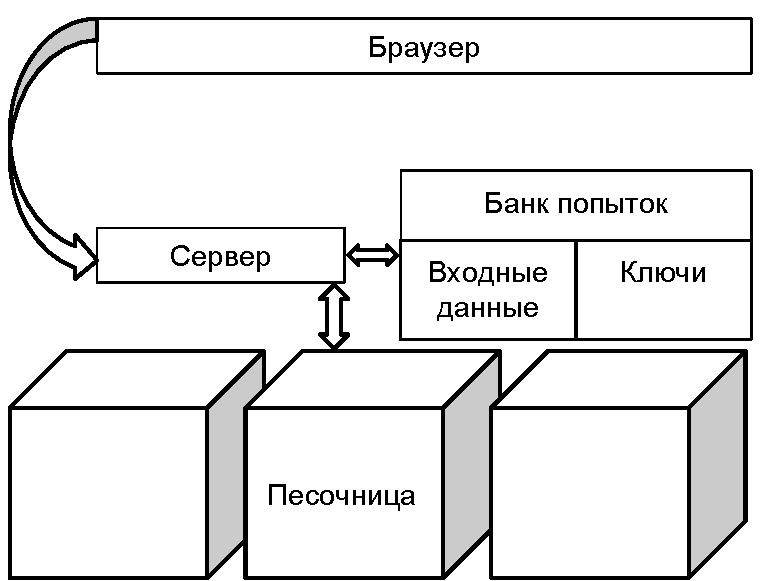
\includegraphics[width=\textwidth]{../res/arch.pdf}
  \caption{Архитектура решения}
\end{figure}

\subsection{Детали реализации}
Для сохранения данных упражнений был выбран формат JSON. Он удобен по
двум причинам. Во-первых, для добавления нового типа упражнений нет
необходимости менять схему базы данных, что позволяет отделить
упражнения от остальной платформы. Во-вторых JSON можно использовать в
качестве формата сообщений, которыми общаются клиент и сервер.

Для реализации серверной части выбран язык Python 3. Это простой и
удобный язык сверхвысокого уровня, главное преимущество которого
заключается в уменьшении затрат на разработку модулей \cite{pyprod}.

Для создания серверной части разработчику модуля упражнения необходимо
определить наследника класса BaseQuiz.

Также при помощи eDSL необходимо описать JSON формат для исходных
данных упражнения, входных данных и ответа.

Клиентская часть реализуется на JavaScript или на CoffeeScript. Для
реализации клиентской части упражнения необходимо определить функции
отрисовки начальных данных для интерфейса редактирования и функции
отрисовки входных данных и ответа для интерфейса решения. Также есть
возможность создавать клиентскую часть упражнения в виде компоненты ember.

\subsection{Инструменты для разработки}
Для упрощения разработки модулей упражнений был разработан ряд
инструментов.

Сервер для разработки, который позволяет запускать упражнения без
Stepic. Сервер автоматически перезагружается при изменении исходного
кода. С его помощью можно проверить как серверную, так и клиентскую
части модуля упражнения.

Шаблон упражнения, при помощи которого можно мгновенно начать
разрабатывать свой модуль.

Документация, опубликована на readthedocs\cite{plugins:doc}.

\section{Реализованные типы упражнений}

С помощью фреймворка в Stepic были разработны следующие типы упражнений:
\begin{itemize}
\item Choice
\item Code
\item Dataset
\item Free Answer
\item Math
\item Number
\item Sorting
\item String
\end{itemize}

\subsection{Примеры конкретных упражнений}
Рассмотрим возможности фреймворка на примере некоторых упражнений.


\begin{description}
\item[Choice] просит студента выбрать среди предложенных вариантов
  ответа правильные. У этого квиза есть много опций -- размер выборки,
  её случайность, количество правильных ответов в выборке. Это
  наиболее часто встречающийся в различных платформах тип квиза из-за
  своей простоты. Однако у него есть свои недостатки -- например,
  студент может просто угадывать ответы. И студент не может придумать
  своё, по настоящему оригинальное решение
  \begin{figure}
    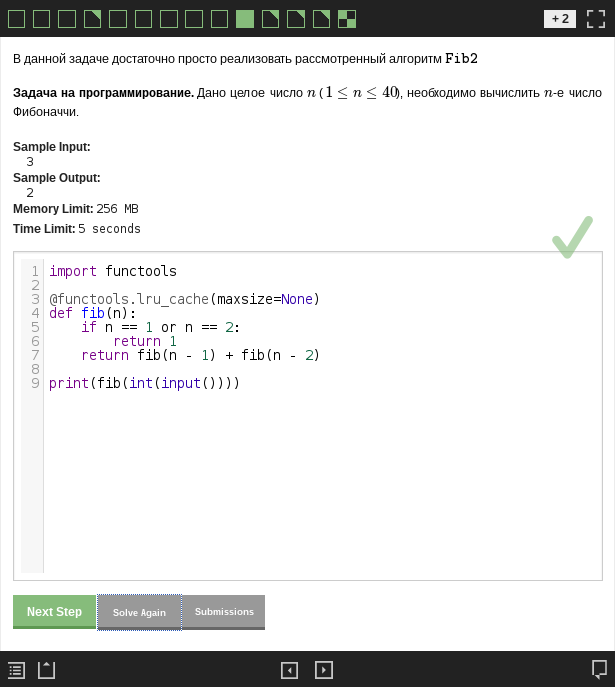
\includegraphics{../res/quiz.png}
    \caption{Пример упражнения (Code)}
  \end{figure}

\item[Dataset] предлагает скачать текстовые входные данные и требует
  текстового ответа. Этот тип упражнений подходить для некоторых
  упражнений на программирование. Он хорош тем, что позволяет
  использовать любой инструмент для решения. Но у этого типа есть и
  недостатки. Размер входных данных не может быть большим, чтобы их
  удобно было скачивать через Интернет. Сложно проконтролировать
  эффективность пользовательского решения. Студенту необходимо иметь
  нужные компиляторы на своей машине.

\item[Code] дополняет dataset. В этом упражнении студент должен
  послать код для решения задачи, которы затем будет исполнен на
  сервере, с замерами времени и памяти. Это удобно для проверки
  эффективности решения, однако необходимо решать задачу на одном из
  поддерживаемых языков программирования(Java, Python, C++, Octave).
\end{description}

\subsection{Использование упражнений на практике}

Созданные упражнения были успешно использованы на практике, при этом в
разных курсах использовались разные типы упражнений.

В курсе "Алгоритмы в биоинформатике" большую часть упражнений
составляли dataset упражнения. Этот тип упражнений оказался наиболее
удобен, так как позволяет делать задачи про обработку больших объёмов
данных, что характерно для биоинформатики, использую при этом любой
язык программирования.

В курсе "Алгоритмы и структуры данных" большую часть упражнений
составляли code и free answer упражнения. Code упражнения оказались
удобны, так как позволяют ограничить решения по времени и памяти, что
необходимо для проверки эффективности реализации алгоритмов. Free
answer упражнения использовались для проверки теоретических задач.

\subsection{Пример использования фреймворка сторонним разработчиком}

С использованием API сторонним разработчиком был создан новый тип
упражнения (admin) для курса по системногу администрированию Linux.

Это упражнение использует сторонний сервис, позволяющий
конфигурировать учебный Linux-сервер с использованием командной
строки.

Задача упражнения --- выполнить настройку определённого ПО на
сервере. Для проверки выполнение задания надо определить набор тестов,
который должен пройти Linux-сервер после конфигурации.

Модуль упражнения admin общается со сторонним сервером по протоколу
HTTP. Интересно, что при разработки API модулей упражнений возможность
коммуникации со сторонними сервисами не рассматривалась, тем не менее
API оказалось достаточно удобным и для этого случая.

Таким образом с помощью фреймворка можно создавать самые разнообразные
типы упражнений.

\section{Изолированное исполнение кода упражнений}

Для многих важных типов упражнений необходимо исполнять потенциально
не безопастный код. Из упражнений, реализованных в Stepic, такими
являются следующие.
\begin{description}
\item[Dataset] Генерация входных данных и проверка ответа происходит
  при помощи кода на языке Python, который вводит автор упражнения.
\item[Code] Также как и в предыдущем случае необходимо выполнять
  Python код автора упражнения. Но для проверки ответа также
  необходимо запустить код студента, который может быть не только на
  Python, но и на другом языке программирования, например на Java или
  Haskell.
\item[Math] В этом упражнении производится сравнение математических
  формул при помощи библиотеки SymPy. Библиотека SymPy может быть не
  безопасна, так как она использует eval.
\item[String] Это упражнение позволяет задавать для проверки
  регулярное выражение. Во многих современных языках программирования
  проверка строки на соответствие регулярному выражению занимает
  экспоненципльное время, что может привести к DOS атаке.
\end{description}

Таким образом возникает необходимость обеспечить изолированное
и ограниченное по ресурсам исполнение кода. Код может быть написан на
языке Python, или на каком-нибудь компилируемом или интерпретируемом
языке программирования.

\subsection{Изоляция}
За основу был взят CodeJail, так как он основывается на безопасном и
удобном для использования Apparmor \cite{Bauer} и удобен для
использоавания из Python.

Тем не менее для использования в Stepic CodeJail был существенно
расширен. Добавлена поддержка различных языков программирования,
улучшены сообщения об ошибках, созданы профили Apparmor для Java,
Octave, Haskell и C++.

\subsection{Масштабирования}
Проверку упражнений важно масштабировать. Особенностью нагрузки
является её неравномерность \cite{breslow2013studying}. Нагрузка
сильно возрастает в последний день сдачи упражнения. В качестве
инструмента для масштабирования была выбрана библиотека Celery, так
как она позволяет масштабироваться эффективно \cite{celery}.

% У заключения нет номера главы
\section*{Заключение}
В результате проделанной работы все поставленные цели были
достигнуты.

Были разработаны следующие типы упражнений: choice, code, dataset,
free answer, math, number, sorting, string. Эти типы упражнений были
успешно использованны в курсах ``Алгоритмы в Биоинформатике'',
``Алгоритмы и Структуры Данных'' и других.

Был разработан API для создания новых типов упражнений в виде
подключаемых модулей. API был документирован. Для облегчения
разработки бы создан небольшой сервер для тестирования модулей. С
использованием API был создан первый сторонний модуль
упражнения. Существующие модули были опубликованы на репозитории на
GitHub.

На основе code jail была создана система безопасного исполнения кода с
возможностью ограничивать и измерять затраченные ресурсы. При помощи
celery достигнуто масшабируемое и распредлённое исполнение кода упражнений.

\bibliographystyle{ugost2008ls}
\bibliography{diploma.bib}
\end{document}


%%% Local Variables:
%%% coding: utf-8
%%% mode: latex
%%% TeX-engine: xetex
%%% End: